%%%%%%%%%%%%%%%%%%%%%%%%%%%%%%%%%%%%%%%%%
% baposter Landscape Poster
% LaTeX Template
% Version 1.0 (11/06/13)
%
% baposter Class Created by:
% Brian Amberg (baposter@brian-amberg.de)
%
% This template has been downloaded from:
% http://www.LaTeXTemplates.com
%
% License:
% CC BY-NC-SA 3.0 (http://creativecommons.org/licenses/by-nc-sa/3.0/)
%
%%%%%%%%%%%%%%%%%%%%%%%%%%%%%%%%%%%%%%%%%

%----------------------------------------------------------------------------------------
%	PACKAGES AND OTHER DOCUMENT CONFIGURATIONS
%----------------------------------------------------------------------------------------

\documentclass[landscape,a1paper,fontscale=0.47]{baposter} % Adjust the font scale/size here

\usepackage{graphicx} % Required for including images
\graphicspath{{figures/}} % Directory in which figures are stored

\usepackage{amsmath} % For typesetting math
\usepackage{amssymb} % Adds new symbols to be used in math mode

\usepackage{booktabs} % Top and bottom rules for tables
\usepackage{enumitem} % Used to reduce itemize/enumerate spacing
\usepackage{palatino} % Use the Palatino font
\usepackage[font=small,labelfont=bf]{caption} % Required for specifying captions to tables and figures

\usepackage{multicol} % Required for multiple columns
\setlength{\columnsep}{1.5em} % Slightly increase the space between columns
\setlength{\columnseprule}{0mm} % No horizontal rule between columns

\usepackage{tikz} % Required for flow chart
\usetikzlibrary{shapes,arrows} % Tikz libraries required for the flow chart in the template

\newcommand{\compresslist}{ % Define a command to reduce spacing within itemize/enumerate environments, this is used right after \begin{itemize} or \begin{enumerate}
\setlength{\itemsep}{1pt}
\setlength{\parskip}{0pt}
\setlength{\parsep}{0pt}
}

\definecolor{lightblue}{rgb}{0.27,0.62,1} % Defines the color used for content box headers
\definecolor{darkgrey}{rgb}{0.27,0.27,0.27} % Defines the color used for content box headers

\begin{document}

\begin{poster}
{
headerborder=closed, % Adds a border around the header of content boxes
colspacing=1em, % Column spacing
bgColorOne=white, % Background color for the gradient on the left side of the poster
bgColorTwo=white, % Background color for the gradient on the right side of the poster
borderColor=lightblue, % Border color
headerColorOne=darkgrey, % Background color for the header in the content boxes (left side)
headerColorTwo=lightblue, % Background color for the header in the content boxes (right side)
headerFontColor=white, % Text color for the header text in the content boxes
boxColorOne=white, % Background color of the content boxes
textborder=roundedright, % Format of the border around content boxes, can be: none, bars, coils, triangles, rectangle, rounded, roundedsmall, roundedright or faded
eyecatcher=true, % Set to false for ignoring the left logo in the title and move the title left
headerheight=0.1\textheight, % Height of the header
headershape=roundedright, % Specify the rounded corner in the content box headers, can be: rectangle, small-rounded, roundedright, roundedleft or rounded
headerfont=\Large\bf\textsc, % Large, bold and sans serif font in the headers of content boxes
%textfont={\setlength{\parindent}{1.5em}}, % Uncomment for paragraph indentation
linewidth=1.5pt % Width of the border lines around content boxes
}
%----------------------------------------------------------------------------------------
%	TITLE SECTION 
%----------------------------------------------------------------------------------------
%
{
\includegraphics[height = 6em]{wits-logo-1.jpg}} % First university/lab logo on the left
{\bf\textsc{ParkSmart - An IoT Parking System for a Smart Campus }\vspace{0.5em}} % Poster title
{\textsc{ Jared Ping \& Lara Timm  \hspace{5pt} \normalsize{School of Electrical \& Information Engineering, University of the Witwatersrand}}} % Author names and institution 
{
\includegraphics[height=7em]{eie-logo.pdf}} % Second university/lab logo on the right


\headerbox{Introduction}{name=introduction,column=0,row=0}{
	The Internet of Things (IoT) is the interconnection of everyday objects, via embedded computing devices and the internet, for the purpose of sending and receiving data. \\
	An IoT parking system enables the availability of parking spaces to be communicated to a user via a mobile application, reducing time and fuel spent searching for a parking space on a daily basis.
	\vspace{1mm}
}

\headerbox{Objectives}{name=objectives,column=0,row=1,below=introduction}{
	\begin{itemize}[leftmargin=13pt]\compresslist
		\item Develop a system which can accurately and reliably communicate parking availability in real time
		\item Provide the most feasible cost effective solution
		\item Keep the system energy efficient, increasing operational time on a single battery charge
		\item Make the system scalable to accommodate any parking lot size
		\item The system should be robust and easy to maintain
		\item Communicate data through a user-friendly mobile application, built using the Android framework
	\end{itemize}

}

\headerbox{System Design}{name=sysdesign1,column=0,below=objectives,bottomaligned=bottom}{ 

	\begin{center}
		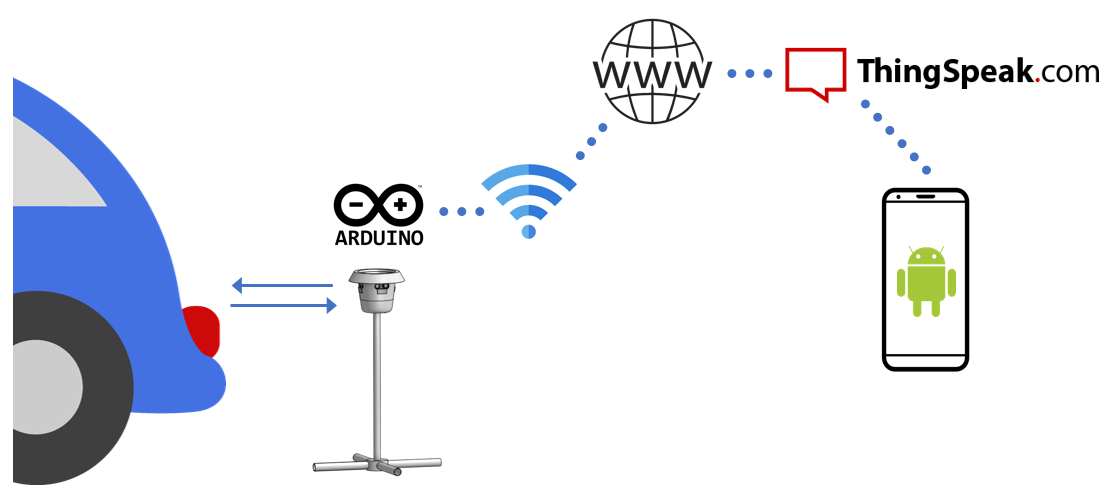
\includegraphics[width=0.9\columnwidth]{Picture2}
		\captionof{figure}{Overall depiction of the implemented system}
	\end{center}

	\textbf{System Features}
		\begin{itemize}[leftmargin=13pt]\compresslist
			\item Parking space availability detection
			\item Empty spaces are communicated to users through a user-friendly mobile application
			\item System updated approximately every 30~s
			\item Functions during active parking hours (7~am - 3~pm)
			\item Fail-safes in place in case of node failures
		\end{itemize}
	
	\textbf{Hardware Setup}
		\begin{itemize}[leftmargin=13pt]\compresslist
			\item Ultrasonic distance measurement sensor
			\item Arduino Nano microprocessor
			\item ESP8266 based Wi-Fi module
			\item 2.4~GHz radio module
			\item 2*AA batteries + 5~V boost converter
		\end{itemize}
	
	
}

\headerbox{System Design (cont.)}{name=sysdesign2,column=1,span=2,row=0}{%,bottomaligned=bottom}{ 
	\begin{multicols}{2}
		
		\textbf{Software Setup}
			\begin{itemize}[leftmargin=13pt]\compresslist
				\item Scalable RF communication mesh is employed \\(refer to Figure 2)
				\item System complexity increases with increasing number of parkings if low cost node design is maintained
				\item Node data is aggregated and uploaded through a single Wi-Fi module (Sink Node)
				\item Optimised data upload through the ThingSpeak MQTT broker
					\begin{itemize}[leftmargin=13pt]\compresslist
						\item Minimal connection and upload time
						\item Small payload size
					\end{itemize}
				\item User-friendly mobile application built for Android
				\item Parking lot data is retrieved by the application through the provided ThingSpeak API
				\item Mobile application automatically refreshes with updated parking bay availability data
			\end{itemize}
		
		\begin{center}
			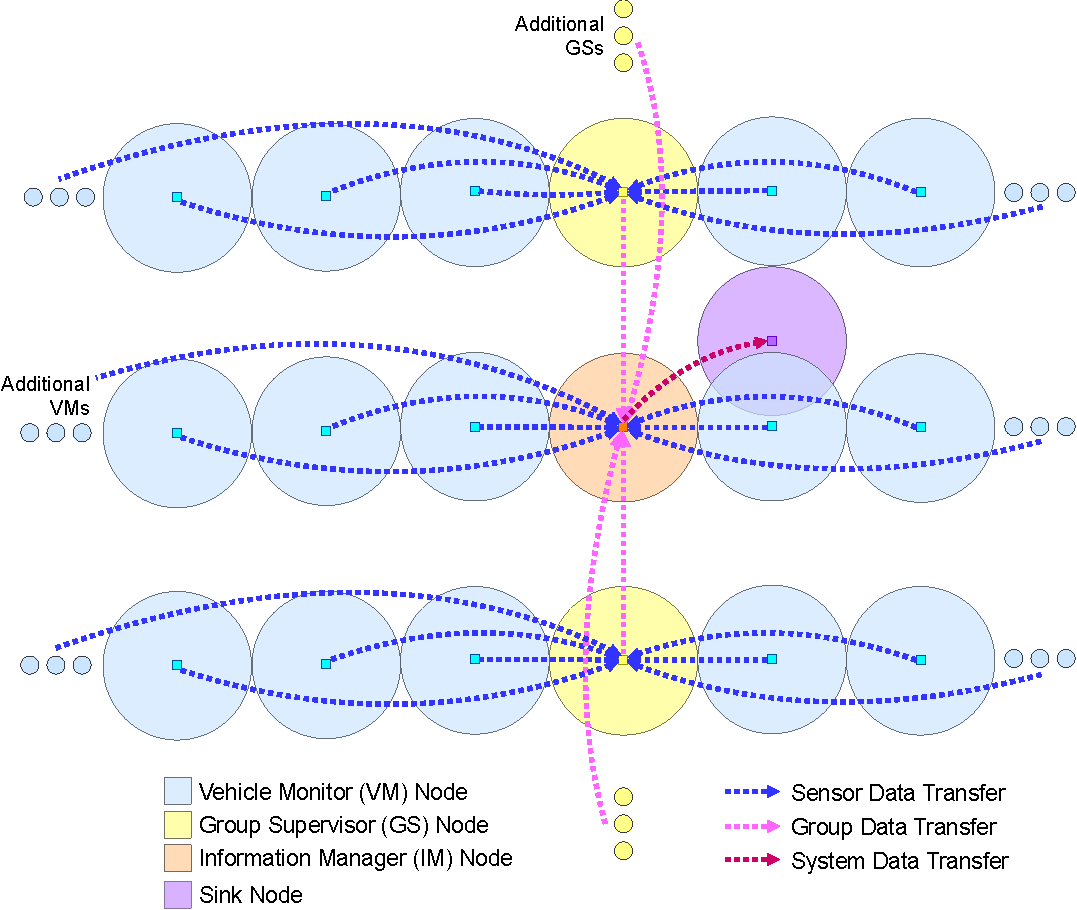
\includegraphics[width=0.8\columnwidth]{mesh-cropped}
			\captionof{figure}{Data retrieval of parking avalability from sensor nodes to sink node}
		\end{center}
	
		\textbf{Smart System Operation}
			\begin{itemize}[leftmargin=13pt]\compresslist
				\item A full cycle incurs an average operation time of approximately 1.6~s (refer to Figure 3)
				\item Mobile application highlights non-transmitting nodes
			\end{itemize}
		
		\vspace{0.5pt}
		
		\begin{center}
			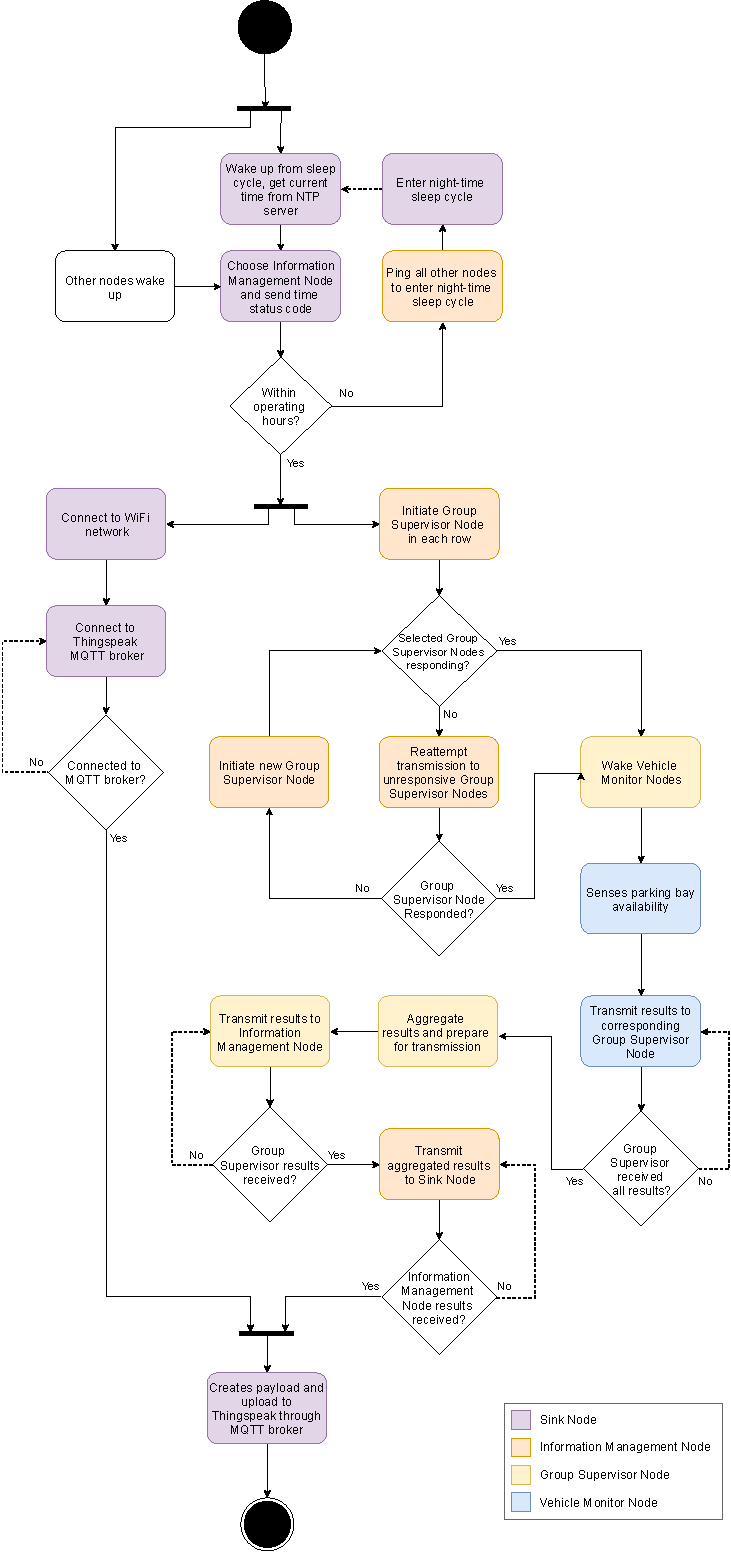
\includegraphics[width=0.9\columnwidth]{flowDiagramBIG-cropped}
			\captionof{figure}{Detailed system interactions between role specific nodes}
		\end{center}
	
	
		
	\end{multicols}
}

\headerbox{Deployment}{name=deployment,column=1,row=1,span=2, below=sysdesign2,bottomaligned=references}{
	\begin{multicols}{2}
		
		\textbf{Construction Specifics} 
		\begin{itemize}[leftmargin=13pt]\compresslist
			\item PCB design for optimized production
			\item 3D printed sensor holders allow customised \\angles per node
			\item Waterproof encasing and tamper-proof lid
			\item Robust stand with runoff resistance
		\end{itemize}
	
	\vspace{1em}
	
		\begin{center}
			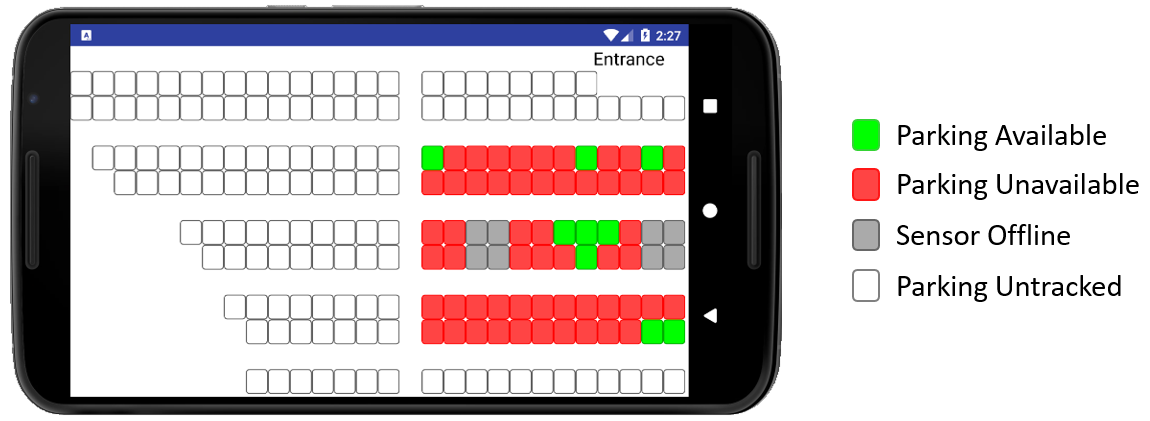
\includegraphics[width=0.67\columnwidth]{app_screenshot2}
			\captionof{figure}{Screenshot of the developed mobile application }
		\end{center}
	
	\end{multicols}
	
}


\headerbox{Results \& Evaluation}{name=deployandeval,column=3,row=0,span=1}{
	
	\textbf{System performance}
		\begin{itemize}[leftmargin=13pt]\compresslist
			\item Estimated system lifetime on a single charge cycle is 276~days
			\item This lifetime is limited by the highest consumption node (refer to Figure~5)
			\item Mobile app data consumption is minimal with a refresh time of 5~s
			\item unupdated requests incur a cost of only 4~kB per request
			\item Data upload cost of implemented system is approximately 3.7~MB per month
		\end{itemize}
	
	\begin{center}
		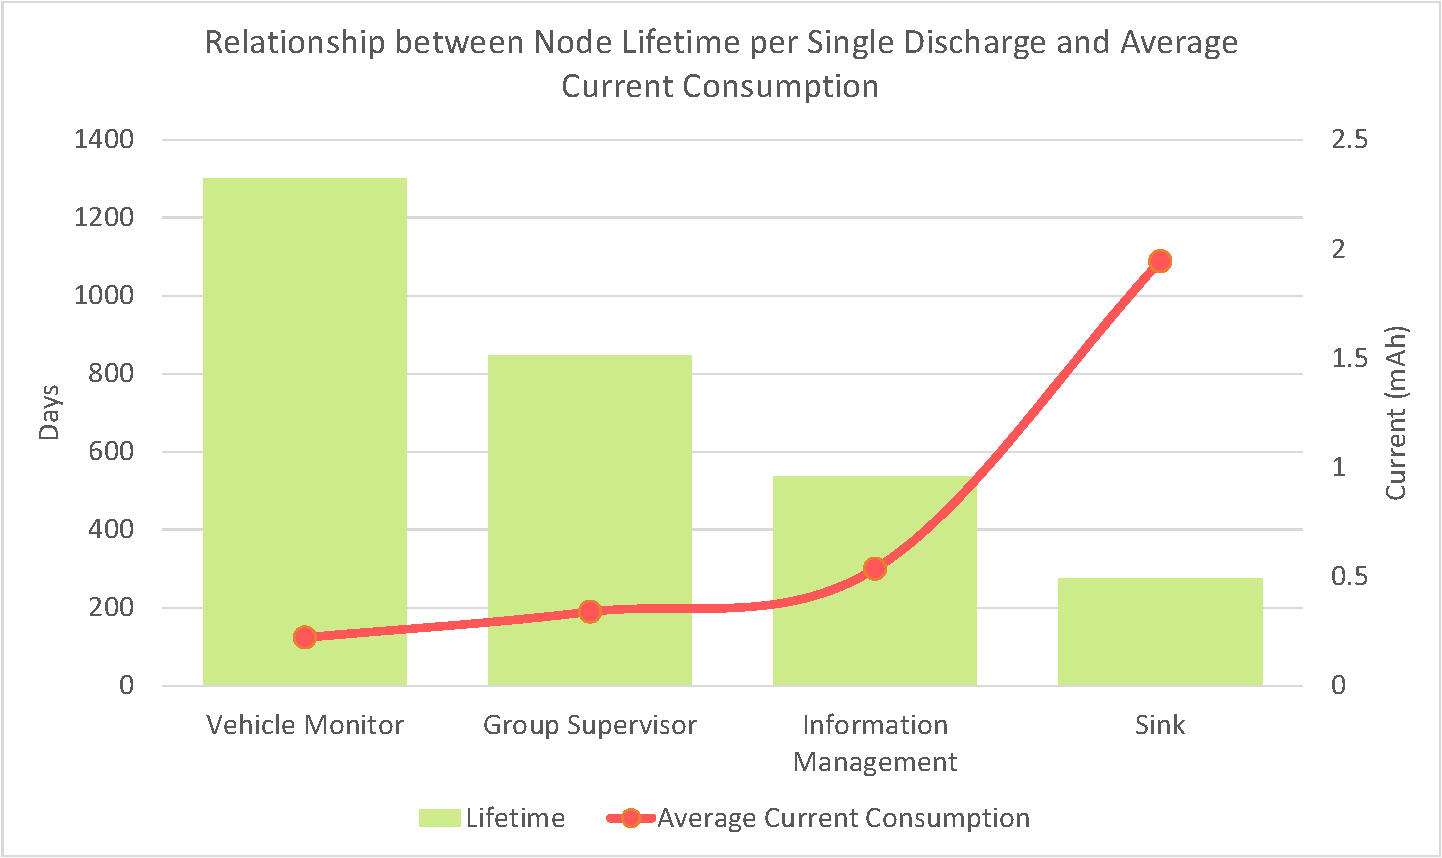
\includegraphics[width=0.7\columnwidth]{lifetime_vs_consumption3}
		\captionof{figure}{Graph depicting energy performance of the system}
	\end{center}
	
	\begin{center}
		\resizebox{1\textwidth}{!}{
		\begin{tabular}{c c c}
			\toprule
			\textbf{Number of Parkings} & \textbf{Payload Size (B)} & \textbf{Monthly Usage (MB)}\\
			\midrule
			1 & 60 & 0.08 \\
			72 & 262 & 3.77 \\
			192 & 582 & 8.38 \\
			\bottomrule
		\end{tabular}
	}
		\captionof{table}{Data consumption of system scaling}
	\end{center}}



\headerbox{Future Work}{name=futurework,column=3,row=1,span=1, below=deployandeval}{
		\begin{itemize}[leftmargin=13pt]\compresslist
		\item An alternative row administrator node row is established if any of the current row administrators go down, allowing negative effects to be dramatically decreased.
		\item Allow sensors to take multiple consecutive readings, use this information to distinguish between the type of object being sensed. This will avoid false positives from pedestrians or other objects crossing the sensor path temporarily.
		\item Small application updates, including the option to manually refresh the parking lot page 
	\end{itemize}
}

\headerbox{Conclusions}{name=conclusion,column=3,span=1,row=3,below=futurework}{
	A prototype IoT-based smart parking system has been designed which comminucates parking availability to  
}

%\headerbox{References}{name=references,column=3,span=1,above=bottom}{
%	
%}

\end{poster}

\end{document}